\section{Internal organization/structure (datapath)}
The internal structure is the one pictured in Figure \ref*{cortexA72conf}. And the details of the blocks are described in section 2.1.1 of source \cite{cortexA72manual}.
\subsection*{Fetch, decode and dispatch units}
\subsubsection*{Instruction Fetch}
Up to 3 instructions are fetched from the L1 instruction memory. The cache has 48KB of size in a 3-way associativity configuration with 64-bits-long cache lines; and optionally, parity bits for error-checking in the data and tag. 
In order to facilitate address prediction and translation, the architecture provides this features: 
\begin{itemize}
	\item {For fast virtual address translation, a Translation Lookaside Buffer (TLB) is with support for pages of sizes 4KB, 64KB, and  1MB.} \label{tlb}
	\item {2-level dynamic Branch Target Buffer (BTB). A static predictor is also provided.}
\end{itemize}


\subsubsection*{Instruction decode}
Types of instructions able to be decoded by the CPU (including)\cite{cortexA72manual}:

\begin{itemize}
	\item {A32: 32-bit wide, aligned on 4-byte boundaries. Both A-profile and R-profile are supported (application and real-time applications respectively) It is the most supported ISA. 
		} \cite{a32instr}
	\item {T32: mixed 32 and 16-bit length instruction set, aiming at lost memory footprint and cost. 
		It's the only ISA supported by type M instructions (specific to microcontrollers)\cite{t32instr}} 
	\item {A64. Instructions semantics similar to A32 and T32, with 31 64-bit general purpose registers; independent from Program Counter and Stack Pointer, and hard-coded zero register.} \cite{a64instr}
	
	This unit performs register renaming to facilitate out-of-order execution; thus removing both WAW and WAR hazards.
\end{itemize}


\subsubsection*{Instruction dispatch}
The dispatch unit controls when the instructions that are decoded are ready to be issued, and afterwards, when the the results are retired. \cite{cortexA72manual}

\subsection*{Functional units for execution and memory access}
This set of functional units is composed by the units for operating with integers, floating point values, and memory accesses. \cite{cortexA72manual}

\subsubsection*{Integer execute}
\begin{itemize}
	\item 2 ALU pipelines.
	\item Integer multiply-accumulate and ALU pipelines.
	\item Iterative integer dividing unit.
	\item Unit for resolution and prediction of branches.
	\item Result forwarding routes.
\end{itemize}

\subsubsection*{Load/Store unit}
This unit is responsible of accessing L1 memory cache and service memory coherency requests with the second cache level (L2).

L1 is a 32KB 2-way associative cache with 64-bits-long lines, and can optionally implement Error Correction Code (ECC)\footnote{The difference between using parity bits in memories and using ECC memory is that, while parity bits helps \textbf{detecting} errors; ECC memory can both \textbf{detect} and \textbf{repair} those errors} for every 32 bits. Apart from the aforementioned TLB (see \nameref{tlb} ), this unit also uses automatic pre-fetching targeting the L1 data cache and L2. \cite{cortexA72manual}

\subsubsection*{Level-2 of cache}
Services the both the data and instruction L1 in case of cache miss, and keeps coherence. For that, it keeps a duplicate of the tag fields of each L1 cache. 
Its size is either 12KB, 1MB, 2MB, or 4MB; with a 16-way associativity with optional ECC data per 64 bits; and a 1024-entry TLB \textbf{for each processor}.
This cache, as explained in the section 7.2 of \cite{cortexA72manual} has a \textit{dirty} bit per line of cache (That is, per 64 bits). For a vision of the whole cache parameters, see table \ref{cachetable}

\subsubsection*{Advanced SIMD and floating-point}
It gives support to ARMv8 advanced SIMD (Simple Input, multiple data) and floating-point operations. Optionally, it is up to the implementation to include an optional cryptography engine, albeit with contractual rights. \cite{cortexA72manual}

\subsubsection*{GIC CPU interface} 
\label{gic}
This unit delivers interrupts to the processor. Examples of interruptions: device signals (device ready, read/write completed, error; battery and power), clock IRQ (for scheduling), exceptions. \cite{cortexA72manual}

\subsection*{Interrupts and debug}


\subsubsection*{Generic Timer}
Provides with the ability to trigger interrupts and trigger events. \cite{cortexA72manual}

\subsubsection*{Debug and trace}
\label{debug}

\begin{itemize}
	\item {ARMv8 debug architecture with slave architecture with debug registers. It provides the programmer with registers for discerning the interrupts \textbf{source}, \textbf{behavior} to apply, and \textbf{routing} to other processors.}
	\item {Performance Monitor Unit: creates statistic data from \textbf{runtime} status of the CPU and the memory}
	\item {Embedded Trace Macrocells: performance of real-time instruction flow tracing.}
	
	\cite{cortexA72manual}
\end{itemize}
\section{Cache memory}

\begin{table}[H]
\caption{Cache parameters for Cortex-A72}
\begin{tabular}{|c|c|c|c|}
	
	\hline 
	Cache level & Sizes available & Associativity & Cache line length \\ 
	\hline 
	Level 1 - Data & 32KB \textbf{per core} & 2-way set assoc. & 64 bits \\ 
	\hline 
	Level 1 - Instruction & 48KBs & 3-way set assoc. &  64 bits \\ 
	\hline 
	Level 2 & 12KB, 1MB, 2MB, or 4MB & 16-way associativity & 64 bits \\ 
	\hline	
\end{tabular} 
\label{cachetable}
\end{table}

In table \ref{cachetable} we have a unified version for all the information regarding cache that was defined previously.

Regarding writing policy, write requests to main memory use as policy \textbf{ Write-back-write-allocate}. This means that updating MM only takes place when cache is \textit{dirty} and prompt to be discarded, and not on MM directly; and upon a miss in cache, the block is brought to the upper levels and allocated there for it to be read or written, and not directly on main memory.
\cite{cortexA72manual} 6.4.1

No access time or bandwidth was found for the cache memories, however, in some implementations, there's information regarding memory controller, therefore cache memory should be faster to access and transfer data from/to. In that specific implementation, the maximum bandwidth for secondary memory is $11.92 GiB/s$; and the most powerful technology to use in this CPU \textit{LPDDR3-1600}, 1600 indicating its frequency in MHz.\cite{mt6797}

\section{I/O support}
The I/O of this architecture is provided by  interfaces with other units or components, being mainly these:

\begin{itemize}
	\item { Memory interface: provides the following advantages: 
		\begin{itemize}
			\item Hardware cache coherency (faster than software).
			\item Transaction ordering for memory.
			\item Management of virtual memory management.
		\end{itemize}
 }
	\item { (Optional) Generic Interrupt Controller, already described in section \ref{gic}.}
	\item { Debug interface, also defined in \ref{debug}; the same as the trace interface. }
	\item { Performance Monitor Unit: provides useful information about the processor when debugging or profiling code. By using six counter can be used to keep track of available events. Those events can be codified and stored in registers of the architecture itself or the APB architecture. \cite{cortexA72manual} 11.2.1
	
	The block diagram is as follows in figure \ref{eventsblock}: 
	
	\begin{figure}[H]
		\centering
		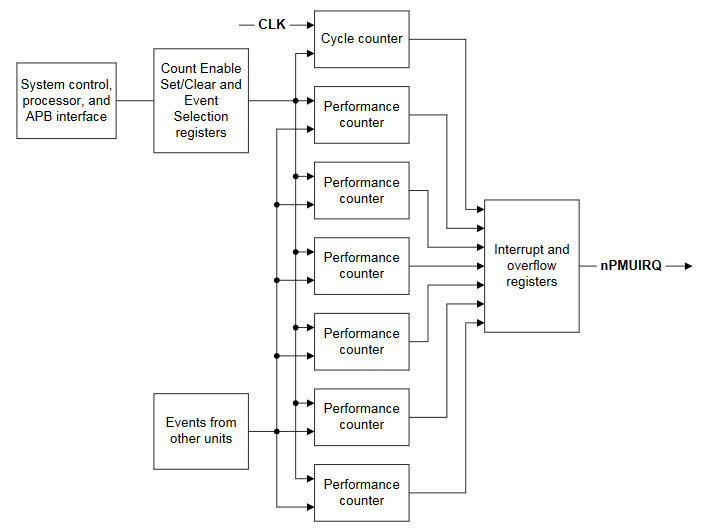
\includegraphics[width=0.7\linewidth]{imgs/eventsblock}
		\caption[]{PMU block diagram}
		\label{eventsblock}
	\end{figure}
}
\end{itemize}